%Laborationsrapport

\documentclass[a4paper,12pt,fleqn]{article}
\usepackage{fixltx2e}
\usepackage[utf8]{inputenc}
\usepackage{graphicx}
\usepackage{sidecap}
\usepackage{fancyhdr}
\usepackage{amssymb,amsmath}
\usepackage[swedish]{babel}
\usepackage[margin=1.5in]{geometry}
\usepackage{abstract}
\usepackage[parfill]{parskip}
\usepackage{tocloft}
\usepackage{adjustbox}
\usepackage{textcomp}
\usepackage[T1]{fontenc}
\usepackage{listings}
\usepackage{xcolor}
%----------------------------------------------------------------
%C-kod formatering

\definecolor{listinggray}{gray}{0.9}
\definecolor{lbcolor}{rgb}{0.9,0.9,0.9}
\lstset{
backgroundcolor=\color{lbcolor},
    tabsize=4,    
%   rulecolor=,
    language=[GNU]C++,
        basicstyle=\scriptsize,
        upquote=true,
        aboveskip={1.5\baselineskip},
        columns=fixed,
        showstringspaces=false,
        extendedchars=false,
        breaklines=true,
        prebreak = \raisebox{0ex}[0ex][0ex]{\ensuremath{\hookleftarrow}},
        frame=single,
        numbers=left,
        showtabs=false,
        showspaces=false,
        showstringspaces=false,
        identifierstyle=\ttfamily,
        keywordstyle=\color[rgb]{0,0,1},
        commentstyle=\color[rgb]{0.026,0.112,0.095},
        stringstyle=\color[rgb]{0.627,0.126,0.941},
        numberstyle=\color[rgb]{0.205, 0.142, 0.73},
%        \lstdefinestyle{C++}{language=C++,style=numbers}’.
}
\lstset{
    backgroundcolor=\color{lbcolor},
    tabsize=4,
  language=C++,
  captionpos=b,
  tabsize=3,
  frame=lines,
  numbers=left,
  numberstyle=\tiny,
  numbersep=5pt,
  breaklines=true,
  showstringspaces=false,
  basicstyle=\footnotesize,
%  identifierstyle=\color{magenta},
  keywordstyle=\color[rgb]{0,0,1},
  commentstyle=\color{Darkgreen},
  stringstyle=\color{red}
  }
  %-----------------------------------------------------------------
  %marginaler

  \renewcommand{\abstractnamefont}{\normalfont\normalsize\bfseries}
  \renewcommand{\abstracttextfont}{\normalfont\small}
  \renewcommand{\headrulewidth}{0pt}
  \renewcommand{\cftsecleader}{\cftdotfill{\cftdotsep}} 
  \setlength{\absleftindent}{0pt}
  \setlength{\absrightindent}{0pt}
  \setlength{\headheight}{15pt}

  \addtolength{\oddsidemargin}{-.5in}
  	\addtolength{\evensidemargin}{-.5in}
  	\addtolength{\textwidth}{1in}


  %-----------------------------------------------------------------
  %header and footer

  \pagestyle{fancy}
  \lhead{
  	\begin{picture}(0,0)
  		\put(5,0){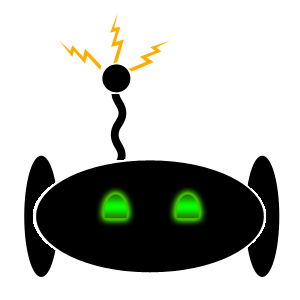
\includegraphics{logotyp.png}}
  	\end{picture}}
	
  \fancyhead[C]{\small{Mapmaster2001}}
  \fancyhead[R]{\small \today}
  \fancyfoot[L]{\small{TSEA56 \\ LIPS Kappa}}
  \fancyfoot[C]{\small{\thepage}}
  \fancyfoot[R]{\small{Projektgrupp 8 \\ mapmaster2001@cyd.liu.se}}

  %-----------------------------------------------------------------

%-------------------------------------------------------------------
%Första sidan

\begin{document}
	\pagestyle{fancy}
\pagenumbering{roman}
	\vspace*{\fill}
		\begingroup
			\begin{center}
				\huge{\textbf{Designspecifikation}}
				\\
				\vspace{5pt}
				\normalsize
				Kandidatprojekt Y - Grupp 8 - VT2014
				\\
				Version 0.1
				\end{center}
		\endgroup
	\vspace*{\fill}
	
	\begin{center} %Börjar centrering 
		Status
		\\
		\vspace{3pt} %Whitespace 3 pts
	    \begin{tabular}{| p{3cm} | p{3cm} | p{3cm} |} %tabell, 4 horizontella |, 3 cm emellan dem.
	    \hline %översta horizontella linjen.
	    Granskad & Av vem & Datum \\ \hline % & -tecken för att "gå till nästa ruta" 
		Godkänd & Av vem & Datum \\ \hline % avslutas med \\ och \hline.

	    \end{tabular}
	\end{center}
	\vspace{2cm}
	\newpage
%-----------------------------------------------------------------
%Projektidentitet
	
	\vspace*{\fill}
		\begingroup
			\begin{center}
				\LARGE{\textbf{PROJEKTIDENTITET}}
				\\
				\footnotesize
				Grupp 8, 2014/VT, MapMaster2001
				\\
				Linköpings tekniska högskola, ISY
				\\
				\vspace{1cm}
	  \begin{tabular}{| p{3cm} | p{4.3cm} | p{2.4cm} | p{3.8cm} |}
	    \hline
		\textbf{Namn} & \textbf{Ansvar} & \textbf{Telefon} & \textbf{E-post} \\ \hline
	    Jens Edhammer & Dokumentanvsvarig (DOK) & 076-030 67 80 & jened502@student.liu.se \\ \hline
		Erik Ekelund & Designansvarig (DES) & 073-682 43 06 & eriek984@student.liu.se \\ \hline
		David Habrman &  & 976-017 71 15 & davha227@student.liu.se \\ \hline 
		Tobias Grundström & Testansvarig (TES) & 073-830 44 45 & tobgr602@student.liu.se \\ \hline 
		Hans-Filip Elo &   & 073-385 22 32 & hanel742@student.liu.se \\ \hline 
		Niklas Ericson & Projektledare (PL) & 073-052 27 05 & niker917@student.liu.se \\ \hline
	    \end{tabular}
		
		\vspace{1cm}
		\textbf{E-postlista för hela gruppen:} mapmaster2001@cyd.liu.se
		\\[0.5cm]
		
		\textbf{Kund}: Mattias Krysander, Linköpings Universitet, 581 83  LINKÖPING, \\
		013-28 21 98, matkr@isy.liu.se \\
		\textbf{Kontaktperson hos kund}: Mattias Krysander, 013-28 21 98,matkr@isy.liu.se 
		\\
		\textbf{Kursansvarig}: Tomas Svensson, 3B:528,013 28 21 59,tomass@isy.liu.se
		\\[0.5cm]
		\textbf{Handledare}: Peter Johansson, 013-28 1345 peter.a.johansson@liu.se

				\end{center}
		\endgroup
	\vspace*{\fill}
\newpage

%-----------------------------------------------------------------
%Innehållsföreteckning

\addto\captionsswedish{\renewcommand{\contentsname}{Innehållsförteckning}}

\tableofcontents
\thispagestyle{fancy}
\newpage

\pagenumbering{arabic}
%-----------------------------------------------------------------
%Kommunikationsmodul


\section{Kommunikationsmodul}
Modul för att hantera kommunikation mellan robotens olika delkomponenter samt med persondatorn via Blåtand. Kommunikationsmodulen som syns i figur 3, kommer att agera master på robotens interna buss. Vid kommunikation mellan övriga moduler, dvs. sensor- och styrmodulen, kommer denna gå via kommunikationsmodulen.
Kommunikationsmodulen kommer alltså att leverera sensordata mellan roboten och mjukvaran som körs på persondatorn.

\subsection{Kommunikationsfall}
Ett par exempel på kommunikationsfall. \\

Kommunikationsmodulen skickar data mellan de olika enheterna. Ett par olika kommunikationsfall demonstreras nedan i flödesdiagrammet i respektive figurer.

Fall 1: Kommunikationsmodulen skickar manuella styrkommandon till styrmodulen,% se figur~\ref{fig:case1flow}.
Fall 2: Sensormodulen signalerar att ny sensordata är redo, se % figur~\ref{fig:case2flow}.\\
Fall 3: Kartdata skickas från kommunikationsmodulen till PC, se % figur~\ref{fig:case3flow}. \\
Fall 4: PC signalerar nödstop, se figur~\ref{fig:case4flow}. \\


\begin{figure}[htp] %Placera här om det finns plats, annars så snart som möjligt, på toppen av en sida.
  \begin{center}
  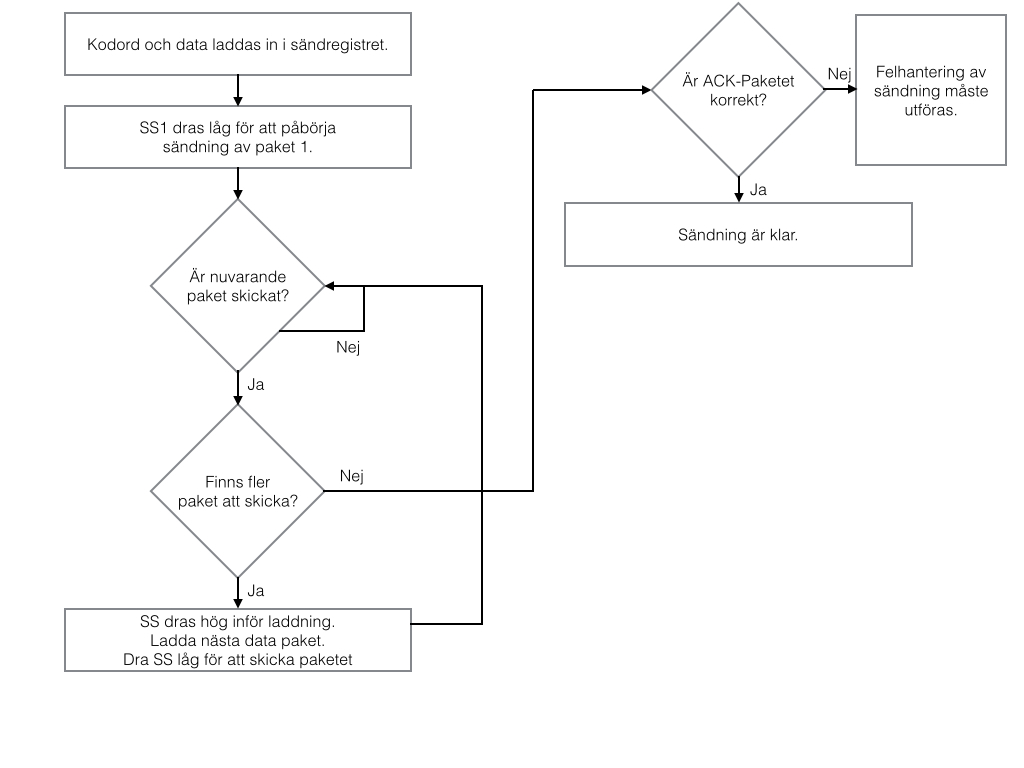
\includegraphics[keepaspectratio=true,scale=0.4]{SPIbild002.jpg}  %skala och filnamn. 
  \end{center}
  \caption{Flödesdiagram för Fall 1.} %figurtext.
  \label{fig:case4flow}
  
\end{figure}

\subsection{Komponenter}
\begin{itemize}
  \item AVR processor av typen ATMega1284
  \item Blåtandsdongel, Firefly, BlueSmirf Gold
  \item LCD-Display
  \item Två stycken knappar
\end{itemize}

\subsection{Buss}
Mellan processorerna kommer SPI-kommunikation att användas. Kommunikationsmodulen agerar master medan styr- och sensormodul agerar slave. 

\subsubsection{Styrord}
Kommunikation kommer starta med att ett styrord skickas. Ett styrord kommer bestå av ett 8-bitars paket (xxxxyyyy). De fyra mest signifikanta bitarna står för kommandot medan de 4 minst signifikanta bitarna står för antalet byte som kommer att följa som argument till kommandot. I tabellerna nedan visas detta mer utförligt. \\

 \begin{tabular}{| p{3cm} | p{3.5cm} |}
	    \hline
		\textbf{xxxx} & \textbf{Kommandonr.} \\ \hline
		0000 & 1 \\ \hline
		0001 & 2 \\ \hline
		... & ... \\ \hline
		1111 & 17 \\ \hline
	    \end{tabular}
		\\

 \begin{tabular}{| p{3cm} | p{3.5cm} |}
	    \hline
		\textbf{yyyy} & \textbf{Antal bytes data} \\ \hline
		0000 & 1 \\ \hline
		0001 & 2 \\ \hline
		... & ... \\ \hline
		1111 & 17 \\ \hline
	    \end{tabular}
		\vspace{0.5cm}
		
		Detta betyder alltså att master kan skicka 16 unika kommandon till respektive slave och varje slave kan skicka 16 unika kommandon till master. Kommandon kan följas av ett upp till och med 17 bytes av data. I händelsen att ett meddelande inte behöver skicka data så skickas en byte nollor.


		Kommandon kommer att kunna betyda olika på de olika processorerna. 0001 kan t ex på slave1 betyda åk rakt längs väggen, på slave2 betyda läs av sensor 3, och på master uppdatera kartabstraktion med följande värden. Om likadana kommandon finns på flera processorer så ska de ha samma kodord på alla processorer som delar kommandot. Ett kommando är reserverat på båda slaves för ett kommando från master som säger du kan skicka information nu. En slave kommer också att kunna skicka ett avbrott till Master för att be om kommunikation. En lista av de olika kodorden finns i appendix. 
		
		På både mottagar- och sändarsida kommer en buffer i form av en länkad lista finnas. Denna lista fylls med data som tas emot och läses från när data ska skickas. 

\subsubsection{Ack-paketets struktur}
Ett sista paket som följer direkt efter datapaketen kommer att skickas. Detta paket är ack-paketet och kommer vara additionen av samtliga datapaketets lägsta bit. Detta ger mottagarsidan en möjlighet att kontrollera att datapaketen mottogs korrekt.
Både sändaren och mottagaren skickar ett sådant ack-paket samtidigt, detta ger oss möjlighet att göra om sändningen direkt, utan att lämna ett eventuellt avbrott. Försök att skicka data utförs tre gånger, om det fortfarande inte lyckats skicka korrekt data, avbryts försöken och lämnas över till felhantering. 

\subsection{LCD-Display}
Sensordata och annan information från roboten kommer att visas på en alfanumerisk-display, närmare bestämt  LCD JM162A. Displayen kommer att kunna visa 2 rader × 16 tecken.
Displayen kommer anslutas till processorn enligt kretschemat i appendix ?. 
Vid varje uppstart kommer initiering av LCD-display göras och då följa nedanstående flödesschema. Varje steg startas med att processorn skickar ett kommando till ingångarna på LCD-displayen. Kommandon finns specificerade i databladet, se (fotnot https://docs.isy.liu.se/twiki/pub/VanHeden/DataSheets/jm162a.pdf). 

\subsubsection{Uppstart}
	
Vid uppstart av systemet kommer LCD-displayen att initieras enligt flödesschemat~\ref{fig:flowlcdstart}

\begin{itemize}
  \item Power ON - sätter på strömförsörjningen
  \item Function set - Sätter överförsdatalängden till 8 bitar och displayläget till 2-rader.
  \item Display ON - slår på displayen och slår på markören. 
  \item Entry mode set - sätter markörens riktning vid skrivning
  \item End - Slut på initieringen
\end{itemize}

\begin{figure}[htp]
	  \begin{center}
	  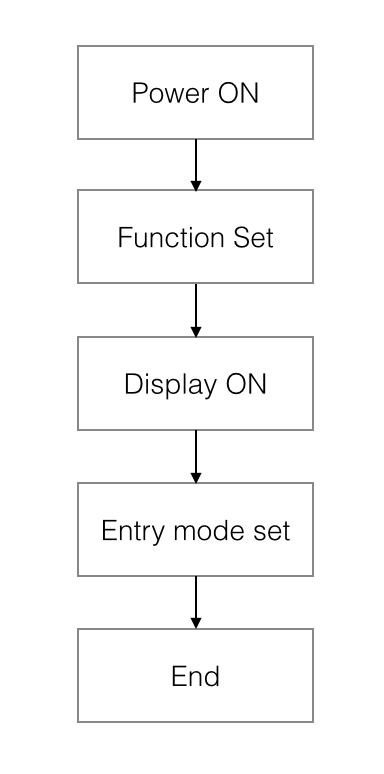
\includegraphics[keepaspectratio=true,scale=0.4]{startup}  %skala och filnamn. 
	  \end{center}
	  \caption{Uppstart av LCD-display} %figurtext.
	  \label{fig:flowlcdstart}
	\end{figure}

\newpage


\subsubsection{Skrivning}

Vid skrivning till LCD-displayen kommer detta ske enligt flödesschemat~\ref{fig:flowlcdwrite}
\begin{itemize}
  \item Start write procedure - Startar skrivning till LCD-displayen
  \item Clear - Rensar hela displayen
  \item Set DDRAM - gör DDRAMet tillgängligt
  \item Write data to RAM - Skrivning av data in till RAM ifrån DDRAM
\end{itemize}

\begin{figure}[htp] %Placera här om det finns plats, annars så snart som möjligt, på toppen av en sida.
  \begin{center}
  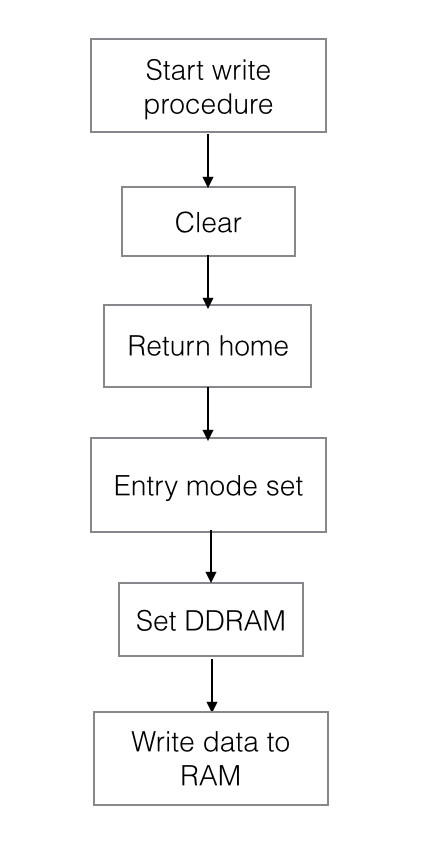
\includegraphics[keepaspectratio=true,scale=0.4]{write}  %skala och filnamn. 
  \end{center}
  \caption{Skrivning till LCD-display} %figurtext.
  \label{fig:flowlcdwrite}
\end{figure}

\subsection{Blåtand}
Blåtandskommunikationen kommer att utföras av ett Firefly-Bluesmirf gold (FBG) modem som parkopplas mot en persondator.
FBG kommer att skicka information till persondator via protokollet RS232 enligt vad som är angivet på Vanheden. 
Se schema i appendixet Scheman för anslutning av TxD och RxD, vilka sköter sändning och mottagning av data.
\subsection{Switchar}
En switch ska styra om roboten exekverar programkod för autonom styrning eller manuell styrning. Ett avbrott signalerar till processorn att den ska byta programkod, avbrottet ligger på pin16 (INT0) se appendix A. 
Av/På-knappen styr strömförsörjningen till samtliga moduler. 

%-----------------------------------------------------------------
%Styrmodul
\section{Styrmodul}


\subsection{Komponenter}
\subsection{Reglering}
\subsubsection{styralgoritmer}
\subsubsection{PD-reglering av styrning}
\subsubsection{kartabstraktion}
\subsection{kartläggninsalgoritm}
\subsection{Brandhärdssökning}
\subsection{Kommunikation}

%-----------------------------------------------------------------
%Styrmodul
\section{Sensormodul}

\subsection{Komponenter}



\subsection{Kod}
Ibland vill man skriva kod, då kan man skriva i annan font. Förslagsvis:
\\ % <--- detta betyder ny rad btw.  

\begin {lstlisting}

for (int i=0; i<iterations;i++)
{
do something hej hej
}
\end{lstlisting}

%---------------------------------------------------------------
\section{Saker som kan vara bra att ha!}

\subsection{Punktlista}
\begin{itemize}
  \item Detta är en punktlista! 
  \item Punktlistor kan innehålla matte. $T_R \leq 10\%$
\end{itemize}

\subsection{Ekvationer}

som vi ser i ekvation~\ref{eq:test} %såhär refererar man till ekvationer och bilder.

\begin{equation}
F(s)= K\frac{\tau_D+1}{\beta\tau+1}\frac{\tau_I+1}{\tau_I+\gamma}	
	\label{eq:test} % glöm inte att ge eran ekvation en label för att kunna referera till den
\end{equation} 

\subsection{Bilder}


\begin{figure}[htp] %Placera här om det finns plats, annars så snart som möjligt, på toppen av en sida.
  \begin{center}
  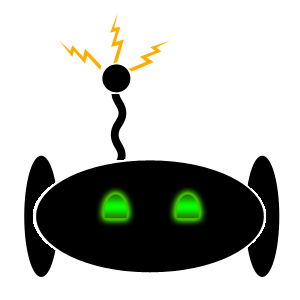
\includegraphics[keepaspectratio=true,scale=0.8]{logotyp}  %skala och filnamn. 
  \end{center}
  \caption{Våran logotyp} %figurtext.
\end{figure}


\end{document}